% !TEX TS-program = pdflatexmk
\documentclass[11pt]{article} 
\usepackage[margin=1in]{geometry} 
\usepackage[parfill]{parskip}% Begin paragraphs with an empty line rather than an indent 
\pdfmapfile{=newtx.map}
\pdfcompresslevel=0
\pdfgentounicode=1
\input glyphtounicode.tex
\usepackage{pdfx} % v 1.6.4 or higher
\InputIfFileExists{glyphtounicode-cmr.tex}{}{}
\InputIfFileExists{glyphtounicode-ntx.tex}{}{}
\usepackage{graphicx} 
\usepackage{url}
\usepackage{trace}
\usepackage{fonttable}
%SetFonts
% newtxtext text and newtxmath
\usepackage{amsmath,amsthm}
\newtheoremstyle{oldplain}
  {\topsep}   % ABOVESPACE
  {\topsep}   % BELOWSPACE
  {\itshape}  % BODYFONT
  {}       % INDENT (empty value is the same as 0pt)
  {\bfseries} % HEADFONT
  {.}         % HEADPUNCT
  {5pt plus 1pt minus 1pt} % HEADSPACE
  {}          % CUSTOM-HEAD-SPEC
\theoremstyle{oldplain}
\newtheorem{oldthm}{Theorem}[section]
\theoremstyle{plain}
\newtheorem{thm}{Theorem}[section]  
%\pdfmapfile{=newtx.map}
\usepackage[osf,p,largesc,theoremfont]{newtxtext}
\usepackage[T1]{fontenc}
\usepackage[varqu,varl]{zi4}
%\traceon
\usepackage{newtxmath}
%\traceoff
%\useosf
\DeclareMathSymbol{\bbZ}{\mathord}{lettersA}{218}
\usepackage{bm}
%SetFonts
\makeatletter
\DeclareMathSymbol{\Sumop}{\mathop}{largesymbols}{"50}
\makeatother
\usepackage{array,booktabs}
\title{New TX font package}
\author{Michael Sharpe}
\date{\today}  % Activate to display a given date or no date

\begin{document}
\maketitle
\section{Introduction}
This package is meant to be a replacement for Young Ryu's {\tt txfonts}. It is  a complete text ({\tt newtxtext}) and math ({\tt newtxmath}) package with roman text font provided by  a Times clone, sans serif based on a \textsf{Helvetica} clone, typewriter faces, plus math symbol fonts whose math italic letters are from a Times Italic clone. As of version 1.4, {\tt newtxtext} no longer depends on {\tt txfonts} but is based on the richer source \textsf{TeXGyre Termes}, but {\tt newtxmath} continues to use the {\tt txfonts} math glyphs with many metric adjustments and some wholesale modifications.

\textsc{Very Important:} The math package changed substantially as of version 1.5, changing a number of glyphs, adding an option to reduce the sizes of large operators, and changing the integral signs to a choice of upright and slanted forms, each available in twelve variants. The new options are {\tt upint} (upright integrals) and {\tt smallerops} (smaller large operators.) Some previously available options may no longer have any effect. The changes are described in detail in the section on math mode options. A summary of the changes in version 1.5 is given in  Appendix 1. 

Version 1.60 likewise has many additions and changes that are summarized in Appendix 2. Most important is that {\tt newtx} is now able to output a PDF/A-1b compliant pdf using {\tt pdflatex}.



This math package works, after possibly replacing its math Roman and Greek letters, with fonts other than Times that are intermediate in weight between Computer Modern and Times. The free font Linux Libertine is one particular target---it is of nearly the same x-height as Computer Modern, but, not being a \emph{modern} font, does not have a high contrast ratio, and so appears  denser than Computer Modern but not as much so as Times. It is meant as a replacement for Times, but  differs from it in many characteristics, more similar to MinionPro than Times, and provides a better range of variants than Times---three weights (regular, semi-bold and bold) rather than just two, and has expert features in all weights: old-style figures, more extensive and more interesting ligatures,  and  small caps. In my opinion, material typeset in Linux Libertine looks better than the corresponding material typeset in Times. This seems especially true on the screen. As of version 1.0, the package also offers support for MinionPro as a math font, but with limitations described in detail below. More recently, an option to provide math support for the \textsf{garamondx} text font package was added. Version 1.55 adds support for the {SticksToo} text fonts, a reworking of the {\tt STIX2} text fonts.

The {\tt newtx} package differs from {\tt txfonts} in the following ways:
\begin{itemize}
\item
the new package is split into separate text and math packages that do not need to be used in conjunction;
\item both text and math packages offer options not present in the original package, described below, including the option to use \textsf{libertine} Latin and Greek letters to replace \textsf{Times}, as well as a similar option \textsf{minion};
\item wide accent glyphs have been corrected (they should have zero depth) so that they no longer collide with the underlying glyph;
\item for those who do not like the integral in \textsf{txfonts}, an emboldened version of the Computer Modern integral is made available, matching the weight of the \textsf{txfonts} symbols;
\item an upright partial derivative symbol has been added, named \verb|\uppartial|;
\item there is now an option to get braces more pleasing to older eyes;
\item macros have been added to bring the calls to Greek symbols more into conformity with \textsc{psnfss} and Mathtime Pro~2;
\item problems using \textsc{ams} macro packages before \textsf{txfonts} are settled;
\item \verb|\coloneq| and \verb|\eqcolon| now point to the correct glyphs;
\item The problem with the {\tt ogonek} accent  and tabular environments (bad definition of \verb|\k|) is fixed: (the definition of \verb|\k| is removed as of version 1.628, being no longer of use);
\item The default encoding for \textsf{newtxtext} is now T$1$, but support is offered also for OT$1$ and LY$1$. As some add-on packages are available only in T$1$, that seems the best current choice.
\item Sans serif is by default taken from TeXGyreHeros, and by default at 90\% of the scale factor (set by {\tt scaled}, default value {\tt1}). The option {\tt helvratio=.98} will change that to 98\%.
\item \verb|\varkappa| $\varkappa$ has been moved from {\tt AMSb} to {\tt lettersA}, and is now accompanied by an upright form \verb|\upvarkappa| $\upvarkappa$ which behaves as it should when using the {\tt frenchmath} option.
\end{itemize}
\section{Text mode options}
Beginning with version 1.4, the text font component of \textsf{newtx} is no longer dependent on the {\tt txfonts}, and is constructed entirely from \textsf{TeXGyre Termes} and some modifications thereof.

The text mode environment invoked by
\begin{verbatim}
\usepackage{newtxtext}
\end{verbatim}
has several options, a number new to version 1.4: you may write
\begin{verbatim}
\usepackage[scaled=.93]{newtxtext}
\end{verbatim}
to load the roman and typewriter text fonts at 93\% of normal size, and the sans serif (\textsf{Helvetica} clone) at scale $0.9*0.93$. This is not of much utility if the package is used with the math package {\tt newtxmath} to which it is already matched, but may be with other math packages. The options
\begin{verbatim}
\usepackage[scaled=.95,helvratio=.96]{newtxtext}
\end{verbatim}
load roman and typewriter text fonts at 95\% of normal size, and the sans serif (\textsf{Helvetica} clone) at scale $0.95*0.96$.

The option \texttt{osf} instructs the text fonts to use old-style figures \oldstylenums{1234567890} rather than the default lining figures $1234567890$. As of version $1.23$, {\tt newtxtext} loads initially with lining figures so the math package uses lining figures in math mode. The option {\tt osf} changes the default to old-style figures in text at the very end of the preamble, forcing the use of old-style figures in text, but not math. In earlier versions, it was necessary to run 
\verb|\useosf| after loading {\tt newtxmath}. This is no longer required. 

If you use the {\tt babel} package, you should load it before {\tt newtxtext}---for example:
\begin{verbatim}
\usepackage[<babel options>]{babel}
\usepackage[osf]{newtxtext}
\end{verbatim}
More generally, the pattern of the preamble should be:
\begin{verbatim}
<encoding options>
[optional] \usepackage{substitutefont} % so you can change babel's fonts
[optional] \usepackage[<babel options>]{babel}
\usepackage[p,osf]{newtxtext}% osf in text, lining figures in math
[optional] redefine the plain theorem style if necessary
<other font loading commands>
\usepackage{newtxmath}
<substitutefont commands>
\end{verbatim}
As an example of a {\tt theoremstyle} definition,
\begin{verbatim}
\usepackage[theoremfont]{newtxtext}
%%% modify the default definition of plain to reduce spacing above and below
\newtheoremstyle{plain}
{0pt}   % ABOVESPACE, extra space above
{0pt}   % BELOWSPACE, extra space below
{\slshape}  % BODYFONT, italic with upright figures and punctuation
{}       % INDENT (empty value is the same as 0pt)
{\bfseries} % HEADFONT
{.}         % HEADPUNCT
{5pt plus 1pt minus 1pt} % HEADSPACE
{}          % CUSTOM-HEAD-SPEC\newtheorem{thm}{Theorem}[section]
\end{verbatim}

Here is a specific example following this pattern, but without {\tt theoremfont}.
\begin{verbatim}
\usepackage[LGR,T1]{fontenc} % spell out all text encodings used
\usepackage[utf8]{inputenc} % 
\usepackage{substitutefont} % so we can use fonts other than those in babel
\usepackage[greek.polutoniko,english]{babel}
\usepackage[largesc,osf]{newtxtext} % 
\usepackage[varqu,varl]{zi4}% inconsolata
\usepackage{cabin}% sans serif
\usepackage[vvarbb]{newtxmath}
\useosf % use oldstyle figures except in math
\substitutefont{LGR}{\rmdefault}{Tempora} % use Tempora to render Greek text
\end{verbatim}

As of version 1.4, there are four normal figure styles: tabular lining, tabular oldstyle, proportional lining and proportional oldstyle, the default figure alignment being \texttt{tabular}. To make \texttt{proportional} the default, use the option \texttt{p} or \texttt{proportional}.

Option {\tt defaultsups} (same effect as {\tt defaultsups=true}) forces the package to use the \LaTeX\ default footnote markers (or, at least, those in force when the package is loaded) instead of those preferred by the package---Times Roman superior figures instead of spindly ordinary Times lining figures reduced to about 70\%. (Footnote markers in minipages use the default lowercase italic alphabetic characters, unless otherwise specified by redefining \verb|\thempfootnote|.) For better control over position and size of footnote markers, use the {\tt superiors} package after loading {\tt newtxtext}. The \verb|\sustyle| font switch and its related \verb|\textsu| macro know not only about figures, but also the lower case letters, including \texttt{egrave}, so that traditional French expressions like \textlf{1}\textsu{i\`ere} may be typeset correctly.

As of version 1.625, there are now denominator figures (aligned to the text baseline) which may be called either with \verb|{\infigures 12345}| {\infigures 12345} or \verb|\textin{6789}| \textin{6789}. Currently, these are available only in regular weight, upright shape. There is a new macro \verb|\textfrac| that builds a fraction from superior figures and denominator figures: e.g., \verb|\textlf{5}\,\textfrac{7}{80}| renders as \textlf{5}\,\textfrac{7}{80}.

Option \texttt{largesc} changes the small cap glyphs from the default petite caps defined in TeXGyre Termes (same size as in txfonts) to a larger size that, in upright shapes, is metrically compatible with Adobe's small caps. These are about 10\% larger than petite caps. For a comparison, \textsc{Small Caps}, {\usefont{T1}{qtm}{m}{sc}Petite Caps}, and \textsc{\textit{Italic Small Caps}}, {\usefont{T1}{qtm}{m}{scit}Italic Petite Caps}.

Option \texttt{adobesc} is only for those who own licenses for \textsf{Adobe Times Small Caps} and install them into the \texttt{ptmsc} package downloaded from \textsc{ctan}. This option loads \texttt{largesc} and substitutes the Adobe glyphs, where available, including their larger Regular and Bold tabular oldstyle figures.

The {\tt theoremfont} option changes the default font used for the {\tt plain} theoremstyle of {\tt amsthm}, keeping italic text but substituting upright figures and punctuation, and, provided you have loaded {\tt amsthm} before {\tt newtxtext}, it will redefine the plain theoremstyle.  For example, with this option, you get theorem statements like this:

\begin{thm}
This is Theorem Italic: text numbers are upright---12345; punctuation is in many cases upright (also, parens, braces \{\} and brackets []). What about question marks and exclamations? Also upright! [These fit better with math mode punctuation and figures, like: for all $x\in[0,1]$, let $f(x)\coloneq \exp(\alpha x)$].
\end{thm}
Compare this to traditional {\tt plain} theoremstyle with the same text:
\begin{oldthm}
This is Theorem Italic: text numbers are upright---12345; punctuation is in many cases upright (also, parens, braces \{\} and brackets []). What about question marks and exclamations? Also upright! [These fit better with math mode punctuation and figures, like: for all $x\in[0,1]$, let $f(x)\coloneq \exp(\alpha x)$].
\end{oldthm}

If you are using another theorem package (e.g., ntheorem, theorem) you will have to add your own descriptors as specified in its documentation and set the body font to \verb|\slshape|.

\section{Spacing issues}
This new version of {\tt newtxtext} has spacing that is a little different, in its default state, from that of the old {\tt newtxtext}. In small part this is due to the finer kerning of TeXGyre Termes, but mostly because the three parameters that govern inter-word spacing are not the same.
\begin{verbatim}
                               txfonts     Termes
fontdimen2 (interword space)   .25em       .25em
fontdimen3 (interword stretch) .15em       .2em
fontdimen4 (interword shrink)  .06em       .1em
\end{verbatim}
That is, {\tt Termes} has the same normal spacing as {\tt txfonts} but its spacing is more flexible in terms of both stretch and shrink. More frequently than not, a paragraph built with {\tt Termes} will occupy more space than the same built with {\tt txfonts}. For this reason, the package offers some ways to change the spacing parameters. This may be important if you are trying to imitate the pagination of a document built using~{\tt txfonts}.

Option {\tt tighter} sets the three fontdimen values to those of {\tt txfonts}.  

Option {\tt looser} sets the three fontdimen values to \verb|{.3em,.2em,.1em}| respectively. 

If you want full control, the options {\tt spacing, stretch, shrink} allow you to modify one or more of the above fontdimens. For example,
\begin{verbatim}
\usepackage[stretch=.15em,shrink=.095em]{newtxtext}
\end{verbatim}

\section{Math mode options}
The package invoked by
\begin{verbatim}
\usepackage{newtxmath}
\end{verbatim}
loads the math part of the {\tt txfonts} (with revised metrics and additional glyphs) and should be loaded \emph{after} the text font and its encoding have been specified, as it uses the text font settings to define how operators, numbers, math accents, \verb|\mathrm|, \verb|\mathbf| etc.\ are rendered. You should also load a Typewriter font so as not to generate mysterious error messages about \textsf{metafont} trying to generate \texttt{ectt10}. The package offers a number of options.
\begin{itemize}
\item {\tt upint} (new as of version 1.5) selects upright integrals---the default shape is slanted. Each shape/size of integral takes one of twelve form, illustrated below in the case of display size slanted integrals.
\[\int\quad\oint\quad\iint\quad\iiint\quad\iiiint\quad\oiint\quad\oiiint\quad\varointclockwise\quad\ointctrclockwise\quad\fint\quad\sumint\quad\sqint\]
named respectively
\begin{verbatim}
\int \oint \iint \iiint \iiiint \oiint 
\oiiint \varointclockwise \ointctrclockwise \fint \sumint \sqint
\end{verbatim}
The three sizes of the upright integrals look like:
\begin{center}
  \begin{tabular}{@{} cl @{}}
    \hline
    Glyph & Command\\ 
    \hline
    $\smallintup$ & \verb|\smallint[up]|\\ 
    $\intup$ & \verb|\int[up]|  \\ 
    $\displaystyle{\intup}$ & \verb|\displaystyle{\int[up]}|\\ 
    \hline
  \end{tabular}
\end{center}
Note that the suffix {\tt up} is not required unless the document's integral style is slanted. You may find the \verb|\smallint| is useful for inline math mode when it is important not to change the line spacing.
\item {\tt smallerops} (new as of version 1.5) causes big operators other than integrals to render up to 20\% less tall, so that displayed formulas may occupy less vertical space. For example, in the following display, the first operator is the usual \verb|\sum|, the second is what you would get with {\tt smallerops}, the third is \verb|\sum| and the fourth is \verb|\smallsum|, the latter being used mainly with inline math. 
\[\sum \Sumop \sum \smallsum\]
Similarly, there are \verb|\smallprod| and \verb|\smallcoprod| which, along with \verb|\smallsum|, are of class {\tt mathop}, unlike their Greek letter equivalents.
\item (New as of version 1.5.) Two macros allow you to change {\tt fontdimen} values in math mode: \verb|\setSYdimens| and \verb|\setEXdimens|, which allow you to change the {\tt fontdimen} parameters for the {\tt symbol} and {\tt extension} fonts respectively. They may be used only in your preamble. Their arguments can be any valid \TeX\ commands to change {\tt fontdimen} values. For example:
\begin{verbatim}
\def\setSYdimens{\fontdimen16\font=2pt\fontdimen17\font=1.15\fontdimen17\font }
\end{verbatim}
Don't use these unless you know what you're doing.
\item {\tt varg} causes the math italic letters \verb|g,v,w,y| to be replaced by versions which are more distinctive---eg, useful for distinguishing math italic \verb|v| from \verb|\nu|;
\item {\tt varvw} causes the math italic letters \verb|v,w| to be replaced by versions which are more distinctive---eg, useful for distinguishing math italic \verb|v| from \verb|\nu|;
\item {\tt libertine} loads different versions of math italic and bold math italic based on \textsf{Libertine} rather than \textsf{Times}---the {\tt varg} and {\tt varvw} options are disabled in this case, as the equivalent variant forms are made available by default;
\item (new in version 1.55) {\tt stix2} loads different versions of math italic and bold math italic based on \textsf{StixTwoMath} rather than \textsf{Times}---the {\tt varg} and {\tt varvw} options are disabled in this case. See the documentation to the {\tt SticksToo} package, which contains more details and some math samples.
\item (new in version 1.60) {\tt ebgaramond} loads different versions of math italic and bold math italic based on \textsf{EBGaramond} rather than \textsf{Times}---the {\tt varg} and {\tt varvw} options are disabled in this case. See the end of Appendix 2 for an example of a preamble.
\item (new as of version 1.629) {\tt noto, notosans} load different versions of math italic and bold math italic based on \textsf{NotoSerif}, \textsf{NotoSans}  rather than \textsf{Times}. There are some intricacies involved, for which there is a separate package, {\tt notomath}, that tries to offer as simple an interface as it was possible for me to devise.
\item (new in version 1.62) {\tt nc, ncf} load different versions of math italic and bold math italic based on \textsf{ScholaX} (\textsf{New Century Schoolbook}) rather than \textsf{Times}---the {\tt varg} and {\tt varvw} options are disabled in this case. The difference is that o[tion {\tt nc} loads math Greek letters from {\tt newtxmath}, while option {\tt ncf} loads math greek from an adaptation of {\tt fourier} Greek.
\item {\tt minion} loads different versions of math italic and bold math italic based on \textsf{MinionPro} rather than \textsf{Times}---the {\tt varg} and {\tt varvw} options are disabled in this case, as the equivalent variant forms are made available by default---see the extended discussion below;
\item {\tt garamondx} loads different versions of math italic and bold math italic based on \textsf{garamondx} rather than \textsf{Times}---the {\tt varg} and {\tt varvw} options are disabled in this case, as the equivalent variant forms are made available by default.
\item {\tt baskervaldx} (or {\tt Baskervaldx}) loads different versions of math italic and bold math italic based on \textsf{Baskervaldx} rather than \textsf{Times}---the {\tt varg} and {\tt varvw} options are disabled in this case, as the equivalent variant forms are made available by default.
\item {\tt baskerville} (or {\tt Baskerville}, or {\tt baskervillef} or {\tt BaskervilleF}) loads different versions of math italic and bold math italic based on \textsf{BaskervilleF} rather than \textsf{Times}---the {\tt varg} and {\tt varvw} options are disabled in this case, as the equivalent variant forms are made available by default.
\item {\tt charter} (or {\tt xcharter}) loads different versions of math italic and bold math italic based on \textsf{XCharter} rather than \textsf{Times}---the {\tt varg} and {\tt varvw} options are disabled in this case, as the equivalent variant forms are made available by default. \textbf{As of version 1.53, Greek letters in all styles are taken from  new alphabets constructed to match the Charter style.}
\item {\tt alty}  is new as of version 1.611, and applies only when math mode uses Charter alphabets. It causes math italic y to be rendered using a rounder shape that is less problematic than the default shape because it lacks the long tail of the XCharter Italic {\usefont{T1}{XCharter-TLF}{m}{it}y}.
\item {\tt noxchvw} (or {\tt noXchvw} is new as of version 1.54, and applies only when math mode uses Charter alphabets. It causes math italic v and w to be rendered using Charter italic glyphs. Use this only if you don't care if math italic v is hard to distinguish from Greek \verb|\nu|.

\item {\tt cochineal}  loads different versions of math italic and bold math italic based on \textsf{cochineal} rather than \textsf{Times}---the {\tt varg} and {\tt varvw} options are disabled in this case. There are two additional options specific to {\tt cochineal}.
\begin{itemize}
\item
Option {\tt cochf} replaces the default short math italic f with the long italic f used in text.
\item Option {\tt cochrho} replaces the default short form of \verb|\rho| with the the long form used in text.
\end{itemize}
\item {\tt utopia} (or {\tt heuristica} or {\tt erewhon}) loads different versions of math italic and bold math italic based on \textsf{Utopia} rather than \textsf{Times}---the {\tt varg} and {\tt varvw} options are disabled in this case, as the equivalent variant forms are made available by default. The Heuristica or Erewhon font package must be installed to use this option. (Erewhon is based on Heuristica, but is 6\% smaller and has more complete figures styles and small cap styles, as well as a variety of smaller figures---superior, inferior, numerator, denominator.)  For example:
\begin{verbatim}
\usepackage[osf]{erewhon} %extension of Utopia
\usepackage[varqu,varl]{inconsolata} % sans typewriter
\usepackage[scaled=.95]{cabin} % sans serif
\usepackage[utopia,vvarbb]{newtxmath}
\end{verbatim}
\item the {\tt libertine} option also replaces both slanted and upright Greek  symbols by the corresponding Libertine glyphs, and similarly for {\tt minion}, {\tt garamondx}, {\tt ebgaramond}, {\tt stix2}, {\tt xcharter} and {\tt cochineal};
\item
{\tt cmintegrals} instructs \textsf{newtxmath} to load a thicker version of the Computer Modern integral in place of the \textsf{newtxmath} default---the txfonts integral (identical to the integral in the Wolfram fonts), which is not to everyone's taste---a consequence is that none of the special forms of \textsf{txfonts} integrals are available;
\textbf{as of version 1.5, this option does nothing, as the new default is slanted integrals.}
\item the combination
\begin{verbatim}
% The next line is no longer needed, as newtxmath Requires it
%\usepackage{amsmath}% loads amstext, amsbsy, amsopn but not amssymb
\usepackage{newtxmath}
\end{verbatim}
causes no error, unlike the same combination with {\tt txfonts}, but does nothing significant. (Recall that {\tt amsmath} is loaded automatically if you use an \textsc{ams} document class such as {\tt amsart} or {\tt amsbook}, as is {\tt amsthm}.) 
%On the other hand,
%\begin{verbatim}
%%\usepackage{amsmath} % no longer needed
%\usepackage[cmintegrals]{newtxmath}
%\end{verbatim}
%allows you to use the forms \verb|\iint|, \verb|\iiint|, \verb|\iiiint| and \verb|\idotsint| defined in {\tt amsmath}, but using the pumped-up Computer Modern integral loaded by {\tt newtxmath}. 
\item If you wish to use \verb|\usepackage{amsthm}|, place it before loading {\tt newtxmath} or the result will  be
\begin{verbatim}
! LaTeX Error: Command \openbox already defined.
\end{verbatim}
\item {\tt uprightGreek} and {\tt slantedGreek} determine the form of Greek alphabet loaded---the default is {\tt uprightGreek}, which loads upright uppercase and slanted lowercase Greek symbols, as is customary in Anglo-American mathematical typesetting. With the option {\tt slantedGreek}, which you might want to use if you cared about ISO standards, all Greek symbols are slanted. No matter which is set, \verb|\Gammaup| (or \verb|\upGamma|) gives you upright \verb|\Gamma|, etc, and \verb|\Deltait|, \verb|\zetait| give you italic (i.e., slanted) versions of those letters. If you are using a text font family with properly constructed OT$1$--encoded versions, then, no matter what you chose as the default shape for upper case Greek letters, \verb|\mathnormal{\Omega}| etc will always produce the slanted version. (The macro \verb|\mathnormal| means essentially ``use the version of the symbol in {\tt letters}''---i.e., the math italic form. This did not always work as expected in versions prior to 1.45.) Currently, this works as expected with {\tt newtxtext} and {\tt libertine}. 
\item Option {\tt frenchmath} sets the default style in math mode for rendering uppercase Roman and Greek letters to upright, and lowercase Greek letters to upright. (Introduced in v.\ 1.28.)
\item The option {\tt cmbraces} instructs {\tt newtxmath} to ignore the brace collections from {\tt txfonts}, substituting a collection based on thickened versions of the Computer Modern braces, which I find much easier to distinguish from other delimiters. This works quite well in regular weight but looks a bit clunky in bold. The option {\tt bigdelims}, which superseded {\tt cmbraces}, is now not necessary---it is the default as of version 1.5.
\item Option {\tt nonewtxmathopt} (or {\tt scale}, a mistake I cannot now erase) causes newtxmath to not make use of the optical math sizes (7{\tt pt}, 5{\tt pt}), as preferred by some.
\item Option {\tt subscriptcorrection} enables the special spacing of some subscripts. (The default is {\tt nosubscriptcorrection}.)
\item The \textsf{newtxmath} package contains three different Blackboard Bold alphabets, where original \textsf{txfonts} contained two. The default, triggered by \verb|\mathbb{}|, takes its glyphs from the font which replaces {\tt msbm} and has the same overall appearance of a hollowed-out text font, which I find neither bold nor blackboard-like. The second option, taken from \textsf{txfonts}, is triggered by \verb|\varmathbb{}|, is more geometric and, in my opinion, preferable but not optimal. The option {\tt varbb} makes \verb|\mathbb{}| synonymous with \verb|\varmathbb{}|. The third option is the double-struck glyphs from the STIX collection. See the expanded discussion below.
\item {\tt noOT1} affects only those text-math combinations where {\tt operators} is defined by default to OT1 with Greek uppercase letters. It causes {\tt operators} to keep the same encoding as in tex, allowing operatornames to use accented charaters, but losing Greek uppercase.
\item {\tt nosymbolsc} causes the package to not load the {\tt symbolsC} fonts, saving  a math family. (This font contains mostly exotic symbols, along with some very useful, commonly used symbols like \verb|\coloneq| $\coloneq$, \verb|\eqcolon| $\eqcolon$, \verb|\notin| $\notin$, \verb|\notni| $\notni$, \verb|\neq| $\neq$, \verb|\nsubset| $\nsubset$ and \verb|\nsupset| $\nsupset$, but these have been moved (virtually) to {\tt lettersA} so they may continue to be used even if you use the option {\tt nosymbolsc}.) If this option is selected, then, as of version 1.53, new definitions are made for the missing negated symbols. The package {\tt centernot} is now required.
\item {\tt amssymbols} (the default) and {\tt noamssymbols} determine whether the {\tt txfonts} versions of the \textsc{ams} symbols ({\tt AMSm}) are loaded---if so, they override previous settings in {\tt amsmath}. If you use the option {\tt noamssymbols}, then \verb|\mathbb{}| is set to mean the same as \verb|\varmathbb{}|. (One advantage of {\tt noamssymbols} is that you save two of your precious math families for other purposes, such as setting a couple of external math alphabets by means of the \textsf{mathalfa} package.) \textbf{Important note:} if you load an AMS class, like {\tt amsart}, then some trickery will be involved. The AMS classes have an option, {\tt noamsfonts} which currently (2017) does not work as advertised, but is fixed in \TeX Live 2018. It is supposed to prevent the loading of {\tt AMSa} and {\tt AMSb}, which waste two slots. The following workaround seems like a reasonable stopgap until then.
\begin{verbatim}
\def\symAMSb{5}
\documentclass[noamsfonts]{amsart} %or other AMS classes
\let\symAMSb\@undefined
\end{verbatim}
This method of loading the AMS class will save you two slots.
\item {\tt libaltvw} has effect only if the libertine option is selected---in this case, it substitutes for math italic v and w hand-crafted versions based on the Libertine upsilon glyphs.
\item{\tt bigdelims} loads a different math extension font and redefines most of the small and big math delimiters to have larger sizes so that, for example, there is more of a distinction between \verb|(| and \verb|\big(| in math mode. If this option is specified, {\tt cmbraces} is ignored. (This option is unnecessary, as of version 1.5.)
\item{\tt liby} has an effect only if the libertine option is selected---with this option, the math italic y is chosen to be Libertine's italic y instead of the default one from txfonts.
\item As of version $1.18$ of {\tt newtxmath} (and version $1.07$ of {\tt newpxmath}) there are new math accents and macros available.
\begin{itemize}
\item
\verb|\widehat| and \verb|\widetilde| have been extended from $3$ to $6$ sizes, and the smallest is now not as wide as in previous versions. In particular, you can now use, eg, \verb|$\widehat{X}^2$|, which gives $\widehat{X}^2$ without the hat colliding with the superscript.
\item The math double bracket delimiters have been moved to another family so their use is less likely to cause a ``too many math families'' error. The ordinary sizes now have their own macros, \verb|\dlb| and \verb|\drb|, giving, eg, $\dlb 0,T\drb$, as commonly used in probability theory.
\item The new macros \verb|\overgroup|, \verb|\undergroup|, \verb|\overgroupra|, \verb|\overgroupla|, \verb|\undergroupra| and \verb|\undergroupla| are intended as replacements for the \verb|\wideparen| and related macros from the \textsf{yhmath} and \textsf{fourier} packages. In fact, \verb|\overgroup| and \verb|\undergroup| are variants of the existing macros \verb|\overbrace| and \verb|\underbrace|, while the suffixes {\tt ra} and {\tt la} signify right arrow and left arrow respectively. The macro \verb|\widering| places a ring centered over an \verb|\overgroup|, not dissimilar from its use in {\tt yhmath}. Example:
\begin{verbatim}
\[\overgroup{ABC}\quad\overgroupra{ABC}\quad\undergroup{ABC}\quad
\undergroupla{ABC}\quad \widering{ABCD}\] 
\end{verbatim}
gives
\[\overgroup{ABC}\quad\overgroupra{ABC}\quad\undergroup{ABC}\quad\undergroupla{ABC}\quad\widering{ABCD}\] 
\end{itemize}
\item As of version $1.23$, the package contains new math accents \verb|\widearc| and \verb|\wideOarc| similar in effect to those from \textsf{fourier} and \textsf{kpfonts}. Example: 
\begin{verbatim}
\[\widearc{BC}\quad\widearc{ABC}\quad\widearc{ABCD}\quad
\wideOarc{BC}\quad\wideOarc{ABC}\quad\wideOarc{ABCD}\]
\end{verbatim}
gives
\[\widearc{BC}\quad\widearc{ABC}\quad\widearc{ABCD}\quad
\wideOarc{BC}\quad\wideOarc{ABC}\quad\wideOarc{ABCD}\]
%\item {largelibfigs} has effect only if the libertine option is selected---with this option, full-sized figures are substituted in math mode for the default Libertine figures, which are about 8\% below Libertine's Capheight.
\item The option {\tt timesmathacc} changes the default selection of math accents from the Roman text font, forcing the use of the heavier Times accents. (Libertine has much lighter accents which can seem to almost disappear under some conditions.) If your language uses accented operator names, do not use this option.
\end{itemize}
\bigskip

\subsection{Bold Math Italic macros}
It can be a little awkward to specify bold math italic letters without using the \texttt{bm} package, which may have some unintended consequences for some users. The option \texttt{useBImacros} enables the definitions of macros of the form \verb|\BIA|---\verb|\BIz| that may be used instead, all based on the macro 
\begin{verbatim}
\DeclareRobustCommand{\BI@}[1]{%
\begingroup\text{\mathversion{bold}$#1$}\endgroup}
\end{verbatim}
following which, the package conditionally defines, e.g.,
\begin{verbatim}
\DeclareRobustCommand{\BIA}{\BI@{A}}
\end{verbatim}
so that \verb|\BIA| works as expected in all math styles (display, text, script, scriptscript). These macros may be copied with minor changes so that other alphabets may be specified similarly.

\textbf{IMPORTANT:} The Libertine text package is now once again named {\tt libertine}, but requires arguments that are different from the original {\tt libertine} package.

\textsc{Example 1:}
\begin{verbatim}
\usepackage[osf]{newtxtext} % T1, lining figures in math, osf in text
\usepackage{textcomp} % required for special glyphs
%\usepackage{amsmath} % not needed, as it is Required by newtxmath
\usepackage[varvf,vvarbb]{newtxmath}
\usepackage{bm} % load after all math to give access to bold math
%\useosf %no longer required if osf specified
\end{verbatim}
\textsc{Example 2:}
\begin{verbatim}
\usepackage[lining,semibold]{libertine} % a bit lighter than Times--no osf in math
\usepackage[T1]{fontenc} % best for Western European languages
\usepackage{textcomp} % required to get special symbols
\usepackage[varqu,varl]{inconsolata}% a typewriter font must be defined
\usepackage{amsmath,amsthm}% must be loaded before newtxmath
\usepackage[libertine,vvarbb]{newtxmath}
\usepackage[scr=rsfso]{mathalfa}
\usepackage{bm}% load after all math to give access to bold math
%After loading math package, switch to osf in text.
\useosf % for osf in normal text
\end{verbatim}

\textbf{Caution:} If your text font lacks an {\tt OT1} encoded version with uppercase Greek, \verb|\mathrm| and \verb|\mathit| applied to Greek letters won't give you what you expect.
\section{Usage with Lua\LaTeX\ and Xe\LaTeX}
As far as I can tell, \textsf{newtxmath} works with both, but requires a very specific loading order and choice of options. Briefly, except for {\tt libertine} text, the math options must all be loaded prior to loading and using {\tt fontspec}. Be aware that some text packages (eg, {\tt cabin}) may contain a line like
\begin{verbatim}
\RequirePackage{fontspec}
\end{verbatim}
which would prevent (``option clash'' error) a subsequent 
\begin{verbatim}
\usepackage[no-math]{fontspec}
\end{verbatim}
unless suppressed by an appropriate option. E.g., 
\begin{verbatim}
\usepackage[type1]{cabin}
\end{verbatim}
prevents the problem with the {\tt cabin} package.

The following examples illustrate some general models, the most unintuitive being the first because it loads a small version, {\tt minlibertine}, of libertine text for use in math mode as numbers, basic symbols and operators.

\textsc{Example 3:}
\begin{verbatim}
%load text components other than libertine text to be used in math
\usepackage[T1]{fontenc}
\usepackage[scaled=.85]{beramono}% used only by \mathtt
\usepackage[type1]{cabin}% used only by \mathsf
\usepackage{amsmath,amsthm}% must be loaded before newtxmath
\usepackage[libertine]{newtxmath}
% loads minlibertine because no other Roman text package was specified
% so that \mathrm and \mathbf also use minlibertine
\usepackage[scr=rsfso]{mathalfa}
\usepackage{bm}% load after all math to give access to bold math
%Now load the otf text fonts using fontspec---won't affect math
\usepackage[no-math]{fontspec} % process with XeLaTeX or LuaLaTeX
\usepackage{libertine}
%\usepackage[osf,semibold]{libertine} for osf in text, semibold as bold
\end{verbatim}
The next example is similar, but in math mode, numbers, basic symbols, operator names, \verb|\mathrm| and \verb|\mathbf| will render with {\tt fbb-LF}, though  math italic and math Greek letters will be from {\tt libertine}. (Note that one specifies the encoding and redefines \verb|\rmdefault|. For reasons I don't yet understand, it may not work to load the font package---ie, don't substitute \verb|\usepackage{fbb}|, as that will mess up bold in the libertine text package.) 

\textsc{Example 4:}
\begin{verbatim}
%load text components other than libertine text to be used in math
\usepackage[T1]{fontenc}
\renewcommand{\rmdefault}{fbb-LF}% Roman font for use in math mode
\usepackage[scaled=.85]{beramono}% used only by \mathtt
\usepackage[type1]{cabin}% used only by \mathsf
\usepackage{amsmath,amsthm}% load before newtxmath
\usepackage[libertine,vvarbb]{newtxmath}
% does not load minlibertine because another Roman text package was specified
\usepackage[scr=rsfso]{mathalfa}
\usepackage{bm}% load after all math to give access to bold math
%Now load the otf text fonts using fontspec---won't affect math
\usepackage[no-math]{fontspec} % process with XeLaTeX or LuaLaTeX
\usepackage{libertine}
\end{verbatim}


\section{Alternate forms of glyphs}
Prior to version 1.5, several math glyphs had alternate forms:
\begin{center}
  \begin{tabular}{@{} llll @{}}
    \hline
    Command & Result &  Alternate Commands & Alternate Forms\\ 
    \hline
    \verb|\emptyset| & $\emptyset$ & \verb|\varnothing, \emptysetAlt|& $\varnothing, \emptysetAlt$ \\ 
    \verb|\forall| & $\forall$ & \verb|\forallAlt| & $\forallAlt$ \\ 
    \verb|\exists| & $\exists$ & \verb|\existsAlt| & $\existsAlt$ \\ 
    \verb|\nexists| & $\nexists$ & \verb|\nexistsAlt| & $\nexistsAlt$ \\ 
    \hline
  \end{tabular}
\end{center}

To use an alternate form throughout your document without changing all occurrences of the usual command, insert something like the following in your preamble after loading \texttt{newtxmath}:
\begin{verbatim}
\let\forall\forallAlt
\end{verbatim}
As of version 1.5, the old {\tt txfonts} versions of \verb|\forall|, \verb|\exists| and \verb|\nexists| have been removed and the {\tt Alt} versions substituted. Both \verb|\forall| and \verb|\forallAlt| generate $\forall$, and similarly with \verb|\exists| and \verb|\nexists|.

\section{Conformity with amsmath}
The {\tt newtxmath} package now contains a \verb|\RequirePackage{amsmath}|, as it uses a number of the macros defined there. To pass options to {\tt amsmath}, you can pass the options as options to \verb|\documentclass|. For example,
\begin{verbatim}
\documentclass[11pt,intlimits]{article}
\usepackage{newtxtext}
\usepackage{newtxmath}
\end{verbatim}
will load {\tt amsmath} with option {\tt intlimits}. As of version 1.14, {\tt newtxmath} respects the {\tt amsmath} macros for placement of limits on integrals.

\section{The {\tt minion} option}
This option allows the use of MinionPro as math letters (Latin and Greek) within  the math font, but there are some caveats:
\begin{itemize}
\item
you must use a recent version of MinionPro (2.00 minimum, 2.12 or higher prefered), such as the version that comes with recent versions of Adobe Reader. The {\tt MinionPro} package must be generated by {\tt FontPro}, and the CTAN package {\tt minion2newtx} must be installed sepately---it is not in \TeX Live. The details are spelled out in the documentation for the {\tt minion2newtx} package.
\end{itemize}

\section{The \TeX\ math font problem}
Math font packages in \LaTeX\ are susceptible to the ``Too many math alphabets'' error, due to exceeding the limit of just sixteen math font families, or mathgroups, as they are called in \LaTeX. Put in oversimplified terms that do however correctly represent how this all works in \textsf{newtxmath}, the following math fonts are always loaded and permanently (if you didn't prevent loading of some features) occupying slots immediately following \verb|\begin{document}|, and others that may be called for in typesetting a mathematical expression can add to the list as the document grows.

\textsc{Always loaded:}
\begin{verbatim}
0: operators
1: letters
2: symbols
3: largesymbols
4: AMSm (a combination of the old AMSa and AMSb)
5: lettersA
6: symbolsC
7: largesymbolsTXA
8: boldoperators
9: boldletters
10: boldsymbols
11: boldlargesymbols
\end{verbatim}
\textsc{Notes:}
\begin{itemize}
\item If using one of the AMS classes (e.g., {\tt amsart}, {\tt amsbook}), you can save two or more math families by adding the option {\tt noamsfonts} in your \verb|\documentclass| call. As of early 2018, This works only with the most recent versions the AMS classes available in both TexLive and MiKTeX. 
\item
The {\tt operators} font is essentially the Roman text font, used for names of operators and as the target for \verb|\mathrm|---its bold version is used as the target for \verb|\mathbf|;
\item {\tt operators} is defined to be the OT$1$ encoded version of the text font in cases where that version is known to contain upright uppercase Greek letters in its forst eleven slots---eg, newtxtext, libertine.
\item if you typeset an expression that, say, calls for a single bold glyph from  {\tt symbolsC}, that costs you an entire new slot, leaving only two remaining;
\item same with, eg, \verb|\mathit|;
\item same with an external Fraktur, Blackboard Bold or Script glyphs;
\item if you run out of math alphabets, look first to dropping {\tt AMSm}  as well as {\tt symbolsC}, which can save you at least two slots;
\item if space is tight, do not call bold versions of the fonts listed above where the bold version is not already loaded, to avoid loading a new mathgroup; 
\item if you absolutely need a letter (not a math symbol) from some math font that would normally cost you another mathgroup, you might consider using as if it were text, with something like
\begin{verbatim}
\mbox{{\usefont{U}{ntxmia}{b}{n} X}}
\end{verbatim}
which allows you to use letter X from {\tt boldlettersA} but without any math features;
\item there is a macro \verb|\ShowMathFonts| in {\tt newtxmath} which may be called at any point in your document, which will provide you a list of the mathgroups currently in use. This can be helpful in figuring out where problems occur. The output lines take the form
\begin{verbatim}
(<fam number>: <internal font id> = <tfm name> [newtx name])
\end{verbatim}

\end{itemize}
\section{Bold math fonts}\label{sec:boldmath}
Every math font in the {\tt txfonts} package, and in the {\tt newtx} package, is accompanied by a bold version. Some usage examples are given below. Generally, one may use either \verb|\boldmath| to change an entire formula to bold, or \verb|\boldsymbol| to change one symbol, but the spacing generally works better after loading the {\tt bm} package and using the \verb|\bm| macro.

The text glyphs dotlessi (\verb|\i|) and dotlessj (\verb|\j|) are rarely needed in actual text---in many fonts, roman dotlessi is very similar to the numeral 1. They are however sometimes needed to build special math glyphs. The following table shows how to generate the mathematical forms of dotlessi and dotlessj. I illustrate with only dotlessi---dotlessj is entirely analogous.

\begin{center}
  \begin{tabular}{@{} llll @{}}
    \hline
    Type & Weight & Command & Result \\ 
    \hline
    Math Italic & Regular & \verb|$\hat{\imath}$| & $\hat{\imath}$ \\ 
    Math Italic & Bold & \verb|$\bm{\hat{\imath}}$| & $\bm{\hat{\imath}}$ \\ 
    Roman & Regular & \verb|$\hat{\textrm{\i}}$| & $\hat{\textrm{\i}}$\\ 
    Roman & Bold & \verb|$\bm{\hat{\textbf{\i}}}$| & $\bm{\hat{\textbf{\i}}}$\\ 
    \hline
  \end{tabular}
\end{center}
\newcommand{\xyvec}[2]{\ensuremath{#1\mkern1.5mu\bm{\textbf{\i}}#2\mkern1.5mu\bm{\textbf{\j}}}}

In math, bold roman characters are often used to indicate vector quantities, and for this one uses constructions like 
\begin{itemize}
\item
\verb|$\mathbf{x}$| produces $\mathbf{x}$;
\item
\verb|$\bm{\mathrm{x}}$| produces $\bm{\mathrm{x}}$ (same as previous but may offer improved spacing);
\item
\verb|$\bm{x}$| produces $\bm{x}$ (not roman);
\item
\verb|$\bm{\hat{\mathbf{x}}}$| produces $\bm{\hat{\mathbf{x}}}$ (with a bold accent);
\item \verb|$\bm{\dot{x}}$| produces $\bm{\dot{x}}$ (bold but not roman);
\item the macro definition
\begin{verbatim}
\newcommand{\xyvec}[2]{%
\ensuremath{#1\mkern1.5mu\bm{\textbf{\i}}#2\mkern1.5mu\bm{\textbf{\j}}}}
\end{verbatim}
allows you to write \verb|\xyvec{x}{+y}| to output $\xyvec{x}{+y}$;
\item \verb|$\bm{\Gamma}$| produces $\bm{\Gamma}$ (bold Gamma);
\item \verb|$\bm{\hat{\Gamma}}$| produces $\bm{\hat{\Gamma}}$ (bold Gamma with bold accent).
\end{itemize}
(The last two assume that you have effectively set the option {\tt uprightGreek}---the default.)

\section{Blackboard bold}
As mentioned briefly above, the package now has a new blackboard bold alphabet built-in, and some new macros to call the non-default versions. To summarize, the problems are:
\begin{itemize}
\item
the default, called by \verb|\mathbb| is quite ugly and indistinct, but does cooperate with the bolding macros \verb|\bm| and \verb|\boldsymbol|;
\item the original variant form called with the macro \verb|\varmathbb| is better, but the macro conflicts with \verb|\bm|. (In fact, the bold version is identical to the regular version, but it is still not right that it conflicts with them.) The problem stems from the part of the definition of \verb|\varmathbb| which allows you to insert an argument with more than one character, like \verb|\varmathbb{ABC}|. Another problem with \verb|\varmathbb| is that it conflicts with {\tt hyperref}---if you use the macro in a moveable argument such as a section heading, you will provoke a \LaTeX\ error message. The solution is to use macros that take a single character as argument, like \verb|\vmathbb{A}| and \verb|\vvmathbb{A}|, which both cooperate with {\tt hyperref}.
\item the third, new, alphabet is borrowed from the STIX fonts---it is sharp and quite clear, geometric in design.  The macro \verb|\vvmathbb| provided to access this alphabet. The new option {\tt vvarbb} effectively makes \verb|\mathbb| mean the same as \verb|\vvmathbb|.
(The reason for including these in the \textsf{newtx} package rather than calling them from the \textsf{mathalfa} package is that \textsf{newtx} leaves very little space for new math symbol fonts and math alphabets, and this way requires no additional such resources.
\item \textbf{Important note:} Under the option {\tt stix2}, there are still three blackboard fonts but the macro \verb|\vmathbb| now points to glyphs from {\tt DSSerif}, a serifed double-struck family that replaces the original variant that is still available under other options. With {\tt stix2}, the {\tt dotlessi} and {\tt dotlessj} glyphs from the {\tt DSSerif} font are available as \verb|$\imathbbs$| and \verb|$\jmathbbs$|, no matter which blackboard bold option you chose.
\end{itemize}
One interesting feature of the new alphabet is that it contains blackboard bold numbers, of which $0$ and $1$ will likely be the most useful, perhaps as operator names. I find $\vvmathbb{1}$=\verb|$\vvmathbb{1}$| useful in specifying an indicator, AKA characteristic function. Here are some examples:

\begin{center}
  \begin{tabular}{@{} llll @{}}
    \toprule
     & Regular & Bold & Remarks \\ 
    \midrule
Default  & \verb|$\mathbb{R}$| $\mathbb{R}$& \verb|$\bm{\mathbb{R}}$| $\bm{\mathbb{R}}$\\ 
Variant 1     & \verb|$\varmathbb{R}$| $\varmathbb{R}$ &  & Bold is same as regular \\ 
$\dots$or     & \verb|$\vmathbb{R}$| $\vmathbb{R}$ &  & Single char.\ argument\\ 
Variant 2 & \verb|$\vvmathbb{R}}$| $\vvmathbb{R}$& \verb|{\boldmath $\vvmathbb{R}$}| {\boldmath $\vvmathbb{R}$} & Make a macro for this! \\ 
%     & $\bm{\mathbb{AB}}$  & $\bm{\vmathbb{A}\vmathbb{B}}$ & $\bm{\vvmathbb{A}\vvmathbb{B}}$ \\ 
    \bottomrule
  \end{tabular}
\end{center}
The macros \verb|\vmathbb| and \verb|\vvmathbb| have been substantially rewritten as of version 1.55 and can now accept strings as arguments rather than just single characters. At some point in time, the \verb|\bm| and \verb|\boldsymbol| macros stopped working with the prior versions of these macros, and that remains a problem with the new versions. If you need only a few blackboard bold symbols, it may be better practice to define macros for each, including bold versions you might need. E.g., the your preamble:
\begin{verbatim}
\let\bbZ\undefined
\DeclareMathSymbol{\bbZ}{\mathord}{lettersA}{218} % Z may not always be in this slot
\end{verbatim}
Then, \verb|\bm| will correctly understand
\begin{verbatim}
\bbZ\;\bm{\bbZ}
\end{verbatim}
and render it as
\[\bbZ\;\bm{\bbZ}\]

\section{Samples from free Times and Libertine packages}
\textsc{TXFONTS:}\\
\begin{verbatim}
\usepackage{txfonts}
\end{verbatim}
\[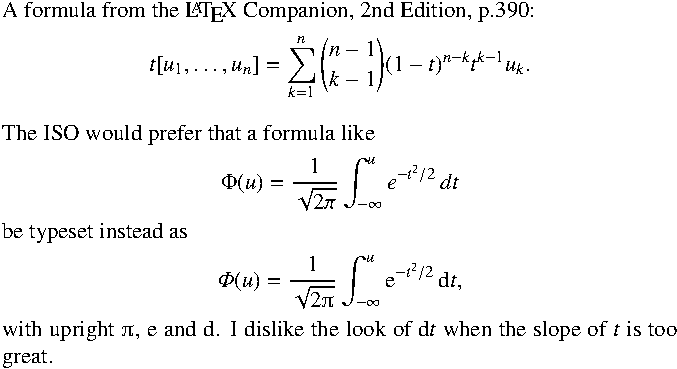
\includegraphics{sample-tx-crop}\]
\begin{itemize}
\item
Complete match between text and math size and weight;
\item first formula much too cramped;
\item upper limit of integral much too close to integral sign;
\item square on $t$ in integrand comes very close to colliding with it;
\item square root in denominator aligned too far right.
\end{itemize}

\vspace{1pc}
\textsc{NEWTXFONTS:}\\
\begin{verbatim}
\usepackage{newtxtext}
\usepackage{newtxmath}
\end{verbatim}
\[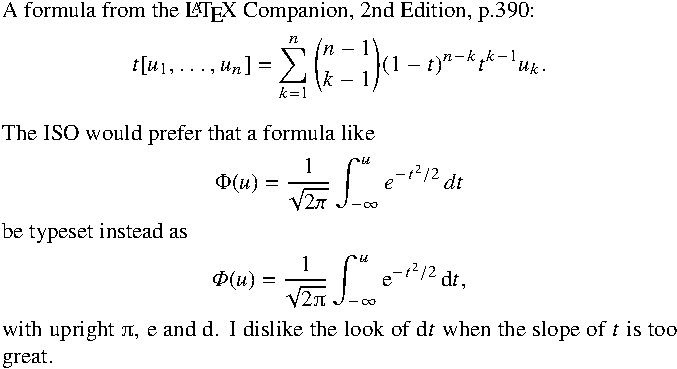
\includegraphics{sample-ntx-crop}\]
\begin{itemize}
\item
Complete match between text and math size and weight;
\item first formula much less cramped;
\item upper limit of integral not too close to integral sign;
\item square not too close to $t$ in exponent;
\item better alignment of square root in denominator.
\end{itemize}

\vspace{1pc}
\textsc{MathTimePro2:}\\
\begin{verbatim}
\usepackage{newtxtext}
\usepackage[lite]{mtpro2}
\end{verbatim}
\[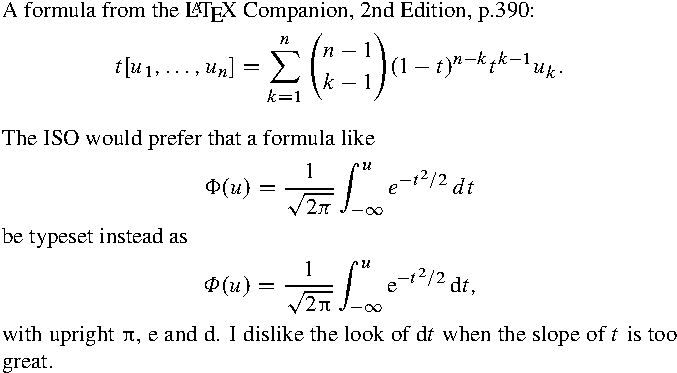
\includegraphics{sample-mtp-crop}\]
\begin{itemize}
\item
Complete match between text and math size and weight;
\item first formula quite spread out;
\item upper limit of integral not too close to integral sign;
\item plenty of space between square and $t$ in exponent.
\end{itemize}

\vspace{1pc}
\textsc{Libertine and MathTimePro2:}\\
\begin{verbatim}
\usepackage{libertine}
\usepackage[T1]{fontenc}
\usepackage[lite]{mtpro2}
\end{verbatim}
\[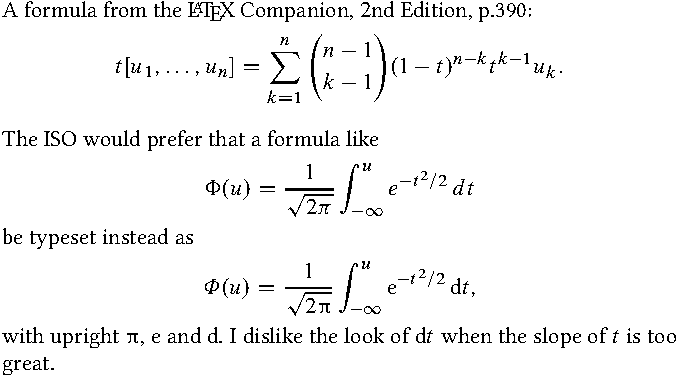
\includegraphics{sample-libmtp-crop}\]
\begin{itemize}
\item
Mismatch of weight between text and math;
\item first formula quite spread out;
\item upper limit of integral not too close to integral sign;
\item plenty of space between square and $t$ in exponent.
\end{itemize}

\vspace{1pc}
\textsc{Libertine and newtxmath:}\\
\begin{verbatim}
\usepackage{libertine}
\usepackage[T1]{fontenc}
\usepackage[libertine]{newtxmath}
\end{verbatim}
\[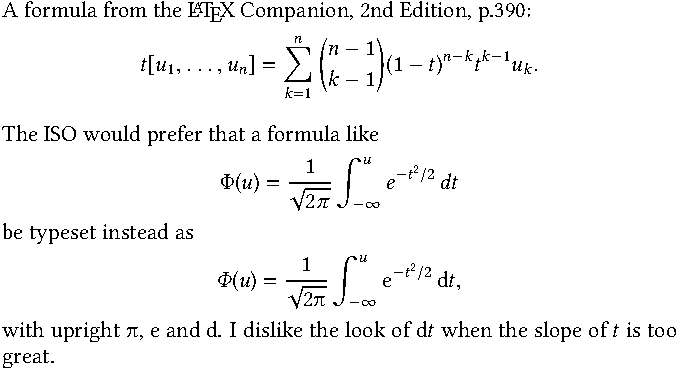
\includegraphics{sample-lib-crop}\]
\begin{itemize}
\item
Very good match between text and math in size and weight;
\item first formula not cramped;
\item upper limit of integral not too close to integral sign;
\item space between square and $t$ in exponent;
\item better alignment of square root in denominator.
\end{itemize}

\vspace{1pc}
\textsc{Mathptmx:}\\
\begin{verbatim}
\usepackage{mathptmx}
\end{verbatim}
\[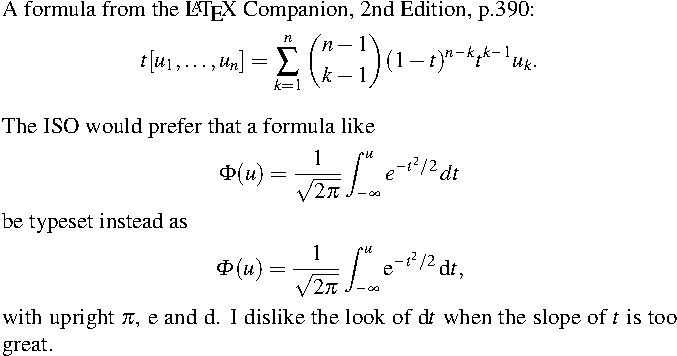
\includegraphics{sample-ptmx-crop}\]
\begin{itemize}
\item
Good match between text and math size and weight, though the summation symbol (from the system {\tt symbol} font) is too small and too dark;
\item first formula well spread;
\item upper limit of integral not too close to integral sign;
\item space between square and $t$ in exponent;
\item there are no upright Greek lowercase letters in this package;
\item good alignment of square root in denominator;
\item infinity symbol not sufficiently large?
\item the package lacks a number of amenities that are present in other packages.
\end{itemize}
\section{Items installed} As well as a collection of PostScript fonts, virtual fonts, font definition files and the central {\tt newtxtext.sty} and {\tt newtxmath.sty} files, the package contains one map file {\tt newtx.map} that must be enabled for the package to function correctly. Its name was changed from {\tt ntx.map} to mirror the package name.) The file \texttt{implementation.pdf} in this distribution provides a manifest of all files installed together with a brief indication of the sources. (This file is somewhat outdated. The file {\tt mathnotes.pdf} adds details about the sources for the math fonts, though it is rather cursory.)

The font files {\tt ntxexmods.pfb} and {\tt ntxbexmods.pfb} were derived from {\tt cmex10.pfb} by FontForgery, thickening the Computer Modern braces to match the weight of the \textsf{txfonts} braces. The pair {\tt ntxexb.pfb} and {\tt ntxbexb.pfb} were similarly derived from {\tt cmsy7.pfb} and {\tt cmex10.pfb} to produce more braces and matching integral signs based on Computer Modern. The {\tt.tfm} files {\tt rtx[b]mio.tfm} are simply unslanted versions of {\tt rtxmi}, from which we construct upright partial derivative symbols.
The last two entries provide us with a way to access custom-encoded versions of {\tt fxlri.pfb} and {\tt fxlbi.map} in order to access some of the unencoded alternate characters---eg, Greek letters, {\tt J.alt} and {\tt v.alt}. The font file \textsf{LibertineTheta-Regular.pfb} was created from the Theta symbol in {\tt fxlri.pfb}, which requires some FontForge help to look correct.

This version contains optical versions of the math italic and symbol fonts at 7\texttt{pt} and 5\texttt{pt}, allowing better rendering in \verb|\scriptstyle| and \verb|\scriptscriptstyle|. 
\section{Appendix 1: Changes made in version 1.5}
\begin{itemize}
\item
The large delimiters have been modified so match the heights in common usage by \texttt{cmex10} and other packages. (Those formerly used by \texttt{newtxmath} were somewhat shorter, resulting in unexpected behavior of \verb|\Big|, \verb|\bigg|, etc.)
\item
The integrals used in previous versions have been discarded and replaced by an upright and a slanted form, the latter being the default. The option {\tt upint} switches to the upright form. (The former option {\tt cmintegrals} now has no effect.) Integrals are of three types: small, textstyle and displaystyle. Each size is available in twelve variants. Assuming slanted (the default) is selected, there are 36 regular-weight forms:
\setlength{\extrarowheight}{8pt}
\begin{center}
  \begin{tabular}{@{} llll @{}}
    \toprule
     Small && Text, Display& \\ 
    \midrule
$\smallint$  & \verb|$\smallint$|& $\int$, $\displaystyle{\int}$& \verb|$\int$|\\ 
$\smalliint$  & \verb|$\smalliint$|& $\iint$, $\displaystyle{\iint}$&\verb|$\iint$|\\ 
$\smalliiint$  & \verb|$\smalliiint$|& $\iiint$, $\displaystyle{\iiint}$& \verb|$\iiint$|\\ 
$\smalliiiint$  & \verb|$\smalliiiint$|& $\iiiint$, $\displaystyle{\iiiint}$& \verb|$\iiiint$|\\ 
$\smalloint$  & \verb|$\smalloint$|& $\oint$, $\displaystyle{\oint}$& \verb|$\oint$|\\ 
$\smalloiint$  & \verb|$\smalloiint$|& $\oiint$, $\displaystyle{\oiint}$& \verb|$\oiint$|\\ 
$\smalloiiint$  & \verb|$\smalloiiint$|& $\oiiint$, $\displaystyle{\oiiint}$& \verb|$\oiiint$|\\ 
$\smallfint$  & \verb|$\smallfint$|& $\fint$, $\displaystyle{\fint}$& \verb|$\fint$|\\ 
$\smallsqint$  & \verb|$\smallsqint$|& $\sqint$, $\displaystyle{\sqint}$& \verb|$\sqint$|\\ 
$\smallsumint$  & \verb|$\smallsumint$|& $\sumint$, $\displaystyle{\sumint}$& \verb|$\sumint$|\\ 
$\smallvarointclockwise$  & \verb|$\smallvarointclockwise$|& $\varointclockwise$, $\displaystyle{\varointclockwise}$& \verb|$\varointclockwise$|\\ 
$\smallointctrclockwise$  & \verb|$\smallointctrclockwise$|& $\ointctrclockwise$, $\displaystyle{\ointctrclockwise}$& \verb|$\ointctrclockwise$|\\ 
    \bottomrule
  \end{tabular}
\end{center}
\item  The overly small delimiters ([\{ in Times are no longer used in math mode, being replaced by bigger versions. The former option {\tt bigdelims} no longer has any effect.
\item There is a new option {\tt smallerops} which chooses smaller renditions (20\% smaller in displaystyle, 10\% smaller in textstyle) of the {\tt bigoperators}:
\begin{verbatim}
\bigsqcup
\bigodot
\bigoplus
\bigotimes
\sum
\prod
\bigcup
\bigcap
\biguplus
\bigwedge
\bigvee
\bigcupdot
\bigcapplus
\bigsqcupplus
\bigsqcapplus
\bigsqcap
\bigtimes
\coprod
\end{verbatim}
\item The dot accents are now taken from a slightly larger series, making available \verb|\dot|, \verb|\ddot|, \verb|\dddot| and \verb|\ddddot|. For best horizontal alignment with other accents, choose the option {\tt timesmathacc} when loading {\tt newtxmath}.
\item New accents have been added and the old vector accent has been replaced. The new accents are:
\verb|\vec|$\quad\vec{}$\\
\verb|\lvec|$\quad\lvec{}$\\
\verb|\lrvec|$\quad\lrvec{}$\\
\verb|\harpoonacc|$\quad\harpoonacc{}$\\
\verb|\lharpoonacc|$\quad\lharpoonacc{}$\\
\verb|\lrharpoonacc|$\quad\lrharpoonacc{}$\\
\verb|\barbar|$\quad\barbar{}$\\
\verb|\bartilde|$\quad\bartilde{}$\\
\verb|\barhat|$\quad\barhat{}$\\
\verb|\tildebar|$\quad\tildebar{}$\\
\verb|\tildetilde|$\quad\tildetilde{}$\\
\verb|\tildehat|$\quad\tildehat{}$\\
\verb|\hatbar|$\quad\hatbar{}$\\
\verb|\hattilde|$\quad\hattilde{}$\\
\verb|\hathat|$\quad\hathat{}$\\
\item New glyphs: (B denotes bigger, S denotes smaller)\\
\verb|\cdotB| $\quad\cdotB$ (cf. \verb|\cdot| $\quad\cdot$)\\
\verb|\cdotBB| $\quad\cdotBB$\\
\verb|\circS| $\quad\circS$ (cf. \verb|\circ| $\quad\circ$)\\
\verb|\bulletS| $\quad\bulletS$ (cf. \verb|\bullet| $\quad\bullet$)\\
\verb|\bulletSS| $\quad\bulletSS$\\
\verb|\bulletSSS| $\quad\bulletSSS$\\
\verb|\primeS| $\quad\primeS$ (cf. \verb|\prime| $\quad\prime$)\\

\item New macros \verb|\setSYdimens| and \verb|\setEXdimens| allow experts to modify some math font dimensions.

\end{itemize}

\def\jj{\mkern-3mu j}

\section{Appendix 2: Changes made in version 1.60}
Versions of {\tt newtx}  dated from September, 2019 (1.60 for {\tt newtxmath} make some quite substantial changes, mostly to math mode. 

\section{Goals}
Spurred by work of Ross Moore to provide means of generating archivable pdf using {\tt pdflatex}, the main goal was to change {\tt newtx} and {\tt newpx} to meet the requirements for satisfying the {\tt PDF/A-1b} standards by using an appropriate preamble involving the {\tt pdfx} package and other unicode mapping files. Making these  changes  gave me the opportunity to organize the source files to make them more manageable in  future revisions. 

A further goal whose time seemed ripe was to rework the  spacing of math letters, both Roman and Greek, so they behaved better in superscripts and subscripts. This did not turn out to be so easy. The problem is illustrated by math italic j. If you don't give it enough extra space on the left, it will likely collide with the D in rendering \verb|$D^j$|. On the other hand, if you do give it enough space on the left, it will look bad as a  subscript, appearing too far right. 

A final goal was to make better use of the remaining space in some of the math fonts by placing some math alphabets in them, avoiding perhaps a waste of those precious sixteen math families.

\section{The important changes}
The following changes were made to both {\tt newtx} and {\tt newpx}.

\subsection{Archivability}
Some of the individual font files from which the math fonts are built turned out to have some fairly minor structural issues. These have all been corrected. The more major issue was the lack of unicode mapping for all characters in the fonts. For the symbol and math extension fonts, this issue was largely solved by Ross Moore's {\tt glyphtounicode} files that are now accessible as part of TeXLive and MiKTeX. The main problem was the math alphabets like math italic, bold math italic, upright Greek and slanted Greek, all of which have now been assigned their own unicode points. For all of these, I constructed new fonts using unicode names for the glyphs, then made \textsf{fontinst} scripts that renamed those unicode values to the original simple names as used in the encoding files so that I could use my old encoding and adjustment files. This exercise has now been carried out for {\tt newtxmath}, {\tt newpxmath}, {\tt newtxmath/libertine}, {\tt newtxmath/cochineal}, {\tt newtxmath/stix2}, {\tt newtxmath/xcharter} and {\tt newtxmath/erewhon.} Each of these can now be considered to have an ``enhanced'' status that allows them to share all the new assets described below. 
 The other packages which may be specified as an option to {\tt newtxmath} (e.g., {\tt baskervaldx, baskervillef}) must be considered for the moment to be ``unenhanced'' and able to share only some of the new assets. In particular, only the enhanced items can generate archivable pdf. 

Also modified were the {\tt sups} fonts in {newtxtext}, where the main issue was unicode mapping. Superior number and some superior letters do have assigned unicode values, but in may cases a more creative approach was needed, and provided once again by Ross Moore. I rebuilt the superior font files using those unicode names, solving that particular problem.

Here is a sample  preamble showing the elements you will need to specify to generate a pdf satisfying the PDF/A-1b standards, as verified by Adobe Acrobat Pro. (Other verification processes may yield different outcomes.)
\begin{verbatim}
\documentclass[noamsfonts]{amsart} % save 2 math families 
\pdfcompresslevel=0 
\pdfgentounicode=1 
\input glyphtounicode.tex 
\usepackage{pdfx} % v 1.6.4 or higher
\InputIfFileExists{glyphtounicode-cmr.tex}{}{} 
\InputIfFileExists{glyphtounicode-ntx.tex}{}{}
\usepackage{newtxtext} %T1 is default encoding
\usepackage[scaled=0.95]{inconsolata}  % typewriter
%\usepackage[leqno]{amsmath} 
\usepackage{amsthm}
\usepackage[vvarbb]{newtxmath} % vvarbb gives STIX Bbb
\end{verbatim}

Version 1.6.3 of {\tt pdfx} from February 2019  mishandles math accents. A fix is now available and will become part of the upcoming {\tt pdfx} v1.6.4.

\subsection{Glyph spacing changes} \textbf{(For enhanced packages only)}I reworked the math italics to improve the rendering of some  superscripts. This affects (a)  parentheses, brackets and braces to inhibit clashes; (b) glyphs like j, f, p, y, \verb|\rho|,  \verb|\beta| and  \verb|\mu| where a long tail could pose problems intersecting with other glyphs; (c) glyphs like such as D, Q and \verb|\Phi| that are round on the right, where interference is most likely to occur with a superscript. Increasing the left side-bearing of j, etc., helps with superscripts but creates an ugly gap when used as subscripts.  


 The {\tt subscriptcorrection} option to {\tt newtxmath} has been corrected and enhanced  so that it now offers a partial solution the subscript spacing problem. I regret that this option is incompatible with xy-pic, both depending on making \verb|_| an active character. {\tt Newtxmath}  will detect if the {\tt xy} package is loaded and disable {\tt subscriptcorrection} if so. You would have to correct such issues by manually inserting a negative \verb|\mkern|. For example, you might put in your preamble something like
 \begin{verbatim}
\def\jj{\mkern-3mu j}
\end{verbatim}
and then use \verb|$x_{\jj}$| instead of \verb|$x_j$|, turning $x_j$ into $x_{\jj}$.

If you do enable {\tt subscriptcorrection}, there is a default correction table in the {\tt sty} file, but the sty file also looks for a file named, e.g., {\tt newtx-subs.tex} if you are using the {\tt newtx} default math letters. There is already such a file located in the {\tt newtx} distribution in the \verb|/tex/latex/| folder. If you wish to make changes to this file, copy the file to your home TeX folder where it will be found by TeX before the one in the distribution. The entries in the file are lines like
\begin{verbatim}
{j}{-3}
\end{verbatim}
each of which will have the same effect as the above macro if the first item in the subscript is j. You can also specify Greek letters with lines like
\begin{verbatim}
{\beta}{-1.5}
\end{verbatim}
The complete list of file names recognized for specifying subscript corrections is:
\begin{verbatim}
newtx-subs.tex
newtx-libertine-subs.tex
newtx-xcharter-subs.tex
newtx-cochineal-subs.tex
newtx-baskervillef-subs.tex
newtx-stickstoo-subs.tex
newtx-garamond-subs.tex
newtx-ebgaramond-subs.tex
newtx-baskervald-subs.tex
newtx-erewhon-subs.tex
newtx-minion-subs.tex
newtx-nc-subs.tex
newtx-ncf-subs.tex
newtx-noto-subs.tex
newtx-notosans-subs.tex
\end{verbatim}

\subsection{New glyphs added} \textbf{(For enhanced packages only)} Math family 1 {\tt (letters)} has been extended from 128 slots to 256, retaining the {\tt OML} encoding of the first 128. Most of additional slots have been allocated to a script font from the old STIX collection and an upright modification of that font.
By default, \verb|$\mathscr{F}$| will produce $\mathscr{F}$.\\
$\bullet$ option {\tt uprightscript} changes the output to {\usefont{OML}{ntxmi}{m}{it}\char201}.\\
In both cases, there are full upper-case and lower-case and {\tt dotlessi}, {\tt dotlessj}. To insert the latter, you can write either \verb|$\mathscr{\imath}$| or \verb|$\imathscr$|, rendered as $\mathscr{\imath}$ in the slanted script case.

The secondary letters font {\tt (lettersA)} and math family 2 {\tt(symbols)} have been rearranged. The first of these continues to have a Fraktur alphabet, but it a modification of its original one, having wider vertical stems and a blacker appearance more in keeping with the weight Times. {\tt Dotlessi} and {\tt dotlessj} have been added and can be specified in math mode by \verb|$\imathfrak$| and \verb|$\jmathfrak$|---\verb|$\mathfrak{\imath}$| also works. There are in addition two subsidiary Bbb alphabets in {\tt lettersA}, specified by the respective options {\tt vmathbb}, {\tt vvmathbb}, and there are corresponding {\tt dotlessi}, {\tt dotlessj} activated by \verb|$\imathbb$|, \verb|$\jmathbb$|, which always render as $\imathbb$, $\jmathbb$ mo matter the choice of which Blackboard Bold Alphabet. If you select one of the options {\tt varbb}, {\tt vvarbb}, you will have Bbb digits 0..9 using, e.g., \verb|$\mathbb{1}$| to get~$\vvmathbb{1}$.

Among the new symbols added are:\\
$\bullet$ \verb|\hslash|, \verb|\hbar|, \verb|\lambdaslash|, \verb|\lambdabar|, \verb|\Zbar|, \verb|\Angstrom| are now constructed from the native glyphs, but only in the enhanced families.\\
$\bullet$ Euler's constant \verb|$\Euler$| ($\Euler$).\\
$\bullet$ Hermitian transpose \verb|\hermtransp| or \verb|\htransp| is used like \verb|$\mathbf{A}^{\htransp}$| ($\mathbf{A}^{\htransp}$). This usage is similar to simple transpose \verb|$\mathbf{A}^{\transp}$| ($\mathbf{A}^{\transp}$).\\
$\bullet$ Independence (in the probabilistic sense) can use \verb|\Perp|, $\Perp$, and there is a new \verb|\nPerp|, $\nPerp$ for the negation.

\subsection{Adaptive vector accent} The \LaTeX\ macro \verb|\overrightarrow| provides a right arrow with adaptive width, but not matching the vector head of {\tt newtxmath}. Likewise, the {\tt esvect} provides a similar service with a choice of vector heads, none of which match {\tt newtxmath}. I've added code to provide a matching adaptive vector accent and which uses the same macro name, \verb|\vv|, as {\tt esvect}.
For a comparison of these vector accents, \verb|$\vec{XY} \vv{XY} \overrightarrow{XY}$| renders as\\ 
$\vec{XY} \vv{XY} \overrightarrow{XY}$.\\ 
$\bullet$ \verb|$\vv{AB}$|  renders as $\vv{AB}$.\\ 
$\bullet$ \verb|$\vv*{AB}{x}$| renders as $\vv*{AB}{x}$. This provides better horizontal spacing of subscripts than \verb|$\vv{AB}_{x}$|, $\vv{AB}_{x}$.\\
$\bullet$  You can also do \verb|$\vv*{AB}{\vv{CD}}$|, which  renders as $\vv*{AB}{\vv{CD}}$.\\
$\bullet$ You can change the vertical space between the arrow and the accentee by means of the package option {\tt vecsep}, whose default value is {\tt .25ex}.

\subsection{Miscellaneous Changes}
\begin{itemize}
\item
The superior letters fonts in {\tt newtx} 
have been extended and all glyphs now have appropriate unicode mappings.
\item
The AMS fonts replacement, {\tt ntxsym} corrects the former misplacement of \verb|\kbbb|, \verb|\daleth|, \verb|\circledR| and \verb|\circledS|.)
\end{itemize}
\newpage
\section{Changed Font Tables}
\subsection{letters}
\fonttable{ntxmi}
\newpage  
\subsection{lettersA}
\fonttable{ntxmia}
\newpage  
\subsection{symbols}
\fonttable{ntxsy}
\newpage 
 
\subsection{A sample newtx-subs.tex}
You may either copy the entire block below, starting with the line \verb|\begin{...| and ending after the line beginning \verb|\end{|
and pasting it into the top of your document before the \verb|\documentclass...| line, which will allow for easy editing and will write the file to the same folder as your document, or make your own file, omitting those outer two lines.

\begin{verbatim}
\begin{filecontents*}{newtx-subs.tex}
{f}{-3}
{j}{-3}
{p}{-1}
{y}{-1}
{A}{-3}
{B}{-1}
{D}{-1}
{H}{-1}
{I}{-1}
{K}{-1}
{L}{-1}
{M}{-1}
{N}{-0.5}
{P}{-1}
{X}{-1}
{\rho}{-1.5}
{\mu}{-1}
\end{filecontents*}
\end{verbatim}
\subsection*{The {\tt ebgaramond} option to newtxmath}
As {\tt ebgaramond} has an x-height considerably smaller than {\tt newtx}, some amount of scaling is useful to bridge the gap. In making the replacement letters, I increased the size of the EBGaramond letters by 5\%, so make some scaling combination that compensates for this. The weights of {\tt ebgaramond} used in the substitutions were regular and semibold. This dictates one of the options used for {\tt ebgaramond}.

\textsc{Example preamble:}\\
\begin{verbatim}
\usepackage[lining,semibold,scaled=1.05]{ebgaramond} 
% Latex BOLD renders with ebgaramond semibold 
\usepackage[T1]{fontenc} % best for Western European languages
\usepackage{textcomp} % required to get special symbols
\usepackage[varqu,varl]{inconsolata}% a typewriter font must be defined
\usepackage{amsmath,amsthm}% must be loaded before newtxmath
\usepackage[ebgaramond,vvarbb,subscriptcorrection]{newtxmath} % STIX Bbb
\usepackage{bm}% load after all math to give access to bold math
\end{verbatim}

\end{document}  